%
% filter.tex -- Kalman-Filter
%
% (c) 2006-2015 Prof. Dr. Andreas Mueller, Hochschule Rapperswil
%
\rhead{Filtern}
\chapter{Filtern} \label{chapter-filtern}

In den vergangenen Kapiteln wurden unter den Voraussetzungen einer
bekannten Verteilung einer einzigen Zufallsvariablen Methoden entwickelt,
die Parameter der Verteilung zu schätzen, und die daraus gewonnenen
Hypothesen gegebenenfalls zu testen.
Überlicherweise musste man dazu
mehrere Beobachtungen der gleichen Zufallsvariablen vornehmen.
In der Praxis kann man jedoch
nicht davon ausgehen, dass man ein System mehrmals beobachten kann.
Im Gegenteil wird sich das System zwischen den Messungen weiterentwickeln,
so dass man jeden Zustand nur ein einziges Mal messen kann.
Die bisherige
Theorie ist auf dieses Problem als zunächst nicht anwendbar.
Da aber in vielen Fällen die zeitliche Entwicklung zum Beispiel durch
Naturgesetze vorgegeben ist, sollte man die bereits erfolgten Messungen
früherer Zustände mit der Systementwicklung verrechnen können und
daraus eine bessere Schätzung des Zustandes ableiten können.
Genau
dies leistet ein Filter: er ermittelt aus neu eintreffenden Messungen
des Systemzustands laufend neue Schätzungen des aktuellen Systemzustandes.
Ziel dieses Kapitels ist zu zeigen, wie man für lineare Systeme\footnote{Diese
Einschränkung ist unbedeutend, da sich praktisch alle Probleme linearisieren lassen.}
einen optimalen Filter berechnen kann.

\section{Ein Einführungsbeispiel}
Als Motivation für die nachstehend zu entwickelnde Filtertheorie betrachten
wir ein System mit einer einzigen Zustandsvariablen $x$, die sich in diskreten
Zeitschritten entwickelt.
Wir haben also mit eine Folge von Zuständen $x_k$ zu tun, wobei
bis auf eine zufällige Störung $x_{k+1}$ mit $x_k$ übereinstimmt,
also $x_{k+1}=x_k+u_k$.
Die Zufallsvariable beschreibt den Systemfehler, wir
nehmen an, dass $E(u_k)=0$ und $\operatorname{var}(u_k)=\sigma^2$.

Den Zustand $x_k$ versuchen wir nun zu schätzen, für jeden Zeitpunkt
$k$ gibt es also eine Zufallsvariable $\hat x_k$, die ein Schätzer für
$x_k$ sein soll.
Da wir davon ausgehen, dass sich $x$ nicht ändert, können wir $\hat x_k$
als eine nur auf den zum Zeitpunkt $k$ bekannten Informationen basierende
Schätzung $\hat x_{k+1|k}=\hat x_k$ verwenden.
Der Erwartungswert von $\hat x_{k+1|k}$ ist $E(x_{k+1|k})=x_{k+1}$, die Varianz
ist
\[
\operatorname{var}(\hat x_{k+1|k})
=\operatorname{var}(\hat x_k)+\operatorname{var}(u_k)=p_k^2+\sigma^2,
\]
wobei wir $\operatorname{var}(\hat x_k)=p_k^2$ abkürzen.

Nun wird zu jedem Zeitpunkt auch eine Messung $z_{k+1}$ mit einem Messfehler
$\operatorname{var}(z_{k+1})=\rho^2$ durchführt.
Auch hier haben wir als
Erwartungswert $E(z_{k+1})=x_{k|k+1}$, wir haben jetzt also zwei Zufallsvariablen
$\hat x_{k+1|k}$ und $z_{k+1}$, die beide Information über den tatsächlichen
Zustand $x_{k+1}$ liefern, allerdings mit unterschiedlichen Varianzen.
Wir
versuchen daher, die Schätzung $\hat x_{k+1}$ als gewichtetes Mittel 
von $\hat x_{k+1|k}$ und $z_{k+1}$ zu bilden
\begin{equation}
\hat x_{k+1}=(1-K)\hat x_{k+1|k}+Kz_{k+1}=\hat x_{k+1|k}+K( z_{k+1} - \hat x_{k+1|k}).
\label{1dimentwicklung}
\end{equation}
Der Gewichtsfaktor $K$ soll so gewählt werden, dass die Varianz von $\hat x_{k+1}$
minimal wird.
Dazu berechnen wir zunächst die Varianz
\begin{align}
\operatorname{var}(\hat x_{k+1})
&=
(1-K)^2\operatorname{var}(x_{k+1|k})+K^2\operatorname{var}(z_{k+1})\notag\\
&=(1-K)^2(p_k^2+\sigma^2)+K^2\rho^2.\label{varianzentwicklung}
\end{align}
Das Minimum kann durch Ableiten nach $K$ und Nullsetzen gefunden werden:
\begin{align*}
\frac{d}{dK}\operatorname{var}(\hat x_{k+1})
=0&=
-2(1-K)(p_k^2+\sigma^2)+2K\rho^2\\
p_k^2+\sigma^2&=K(p_k^2+\sigma^2+\rho^2)\\
K&=\frac{p_k^2+\sigma^2}{p_k^2+\sigma^2+\rho^2}
\end{align*}
Damit wird die Schätzung $\hat x_{k+1}$
\[
\hat x_{k+1}=\frac{\rho^2}{p_k^2+\sigma^2+\rho^2}\hat x_k+\frac{p_k^2+\sigma^2}{p_k^2+\sigma^2+\rho^2}z_{k+1}
\]
Ebenso kann man jetzt die Varianz $\operatorname{var}(\hat x_{k+1})=p_{k+1}^2$
mit (\ref{varianzentwicklung}) berechnen.
Insgesamt haben wir also folgenden
Satz gewonnen

\begin{satz}
Sei $x_k$ eine Folge von Zufallsvariablen, für die $x_{k+1}=x_k+u_k$ gilt, wobei
$u_k$ eine Zufallsvariable mit Erwartungswert $0$ und Varianz $\sigma^2$ ist.
Sei
ausserdem $z_{k+1}$ eine Folge von Messungen von $x_{k+1}$, d.~h.~$E(x_{k+1})=E(z_{k+1})$
und $\operatorname{var}(z_{k+1})=\rho^2$.
Weiter sei der Anfangszustand $x_0=x$ bekannt.
Die Folgen $\hat x_k$ und $p_k^2$, definiert durch die Anfangswerte
$\hat x_0=x$ und $p_0^2=0$ und die Iterationsgleichungen
\begin{align*}
K&=\frac{p_k^2+\sigma^2}{p_k^2+\sigma^2+\rho^2}\\
\hat x_{k+1}&=\hat x_k + K ( z_{k+1} - \hat x_k)\\
p_{k+1}^2&=(1-K)^2(p_k^2+\sigma^2)+K^2\rho^2,
\end{align*}
ergeben die bestmögliche Schätzung $\hat x_k$ von $x_k$ mit
einem mittleren quadratischen Fehler $p_k^2$.
\end{satz}
Der Gewichtsfaktor $K$ heisst Kalman Filter Faktor.
Ist $K$ gross, wird der
Schätzwert $\hat x_{k+1}$ vor allem durch die Messung bestimmt, ist er
klein, hat die bisherige Schätzung $\hat x_k$ mehr Gewicht.
$K$ wird gross,
also nahe bei $1$, wenn, $\rho^2$ sehr klein ist, wenn also die Messung
sehr genau ist.
In diesem Fall wird auch $p_{k+1}^2$ vor allem durch die
die Grösse $K^2\rho^2$ bestimmt, die Schätzung $\hat x_k$  ist also
ähnlich präzise Messung.
Ist die Messgenauigkeit dagegen gering,
wird die Iteration von einem einmal gefundenen Schätzwert $\hat x_k$
nur in kleinen Schritten abrücken.
Dabei besteht die Gefahr, dass
der Fehler $p_k^2$ stark anwächst, wen nämlich $\sigma^2$ zu gross
ist, kann es geschehen, dass $p_{k+1}^2>p_{k}^2$, so dass der Filter
mit der Zeit immer ungenauer wird.
Daher ist es wichtig, einerseits
eine möglichst gut zutreffende Systembeschreibung zu haben und andererseits
den Systemzustand möglichst genau zu messen.

\section{Problemstellung}
Im Einführungsbeispiel wurde ein eindimensionales System betrachtet,
welches sich nicht verändert.
Im Allgemeinen wird ein System durch
mehrere Variablen beschrieben, die sich in der Zeit verändern.
in diesem Abschnitt wollen wir die Problemstellung des eindimensionalen
Problems auf mehrdimensionale Systeme verallgemeinern.

\subsection{System und Beobachtung}
Zwei Positionsmessung im zeitlichen Abstand $\Delta t$
bei einem Fahrzeug, welches selbständig
in seiner Fahrbahn bleiben soll, können sich bis auf Messfehler um höchstens
$v\Delta t$ unterscheiden, wenn sich das Fahrzeug mit Geschwindigkeit $V(t)$
quer zur Fahrtrichtung bewegt.
Insbesondere würden wir für die zweite
Messung ungefähr den Wert $E(X(t+\Delta t)) = X(t) + V(t)\Delta t$
erwarten.
Hier haben wir unser Wissen über das System einfliessen lassen.

Offensichtlich ist es also möglich, eine gute Voraussage über den
zukünftigen Zustand $X(t+\Delta t)$ zu machen, wenn $X(t)$ und $V(t)$
bekannt sind.
Natürlich wird diese Voraussage nicht mit der tatsächlichen
Messung zur Zeit $t+\Delta t$ übereinstimmen.
Zum einen werden unweigerlich
neue Messfehler auftreten, zum anderen basiert die Voraussage ja bereits
auf Daten, die mit einem Messfehler behaftet sind.
Die Voraussage ist also
ebenfalls eine Zufallsvariable, die jedoch auf der Kenntnis eines früheren
Zustands des Systems basiert.

Wir modellieren dieses Problem jetzt für den Fall konstanter Zeitschritte.
Den Zustand des Systems betrachten wir als Vektor $x_k\in\mathbb{R}^n$,
wobei $k\in\mathbb{N}$.
Diese Vektoren sind nicht vollständig beobachtbar,
nur ein Abbild davon ist messbar.
Grundsätzlich müssten wir also eine
bestimmte Funktion auf $x_k$ anwenden, um die Messgrössen zu finden,
für die meisten praktischen Anwendungen genügt es, eine lineare Abbildung
zu verwenden.
Es gibt also eine Matrix $H_k$, welche die beobachteten
Grössen $z_k=H_kx_k$ bestimmt.

Die Zeitentwicklung des Systems muss aus einem Zustand $x_k$ den nächsten
Zustand $x_{k+1}$ berechnen.
Bei einem
einfachen System mit der Bewegungsgleichung
\[
\frac{dx(t)}{dt}=ax(t)
\]
gilt zum Beispiel $x(t_2)=e^{a(t_2-t_1)}x(t_1)$, d.~h.~der Zeitschritt
kann durch Multiplikation mit einer Zahl $e^{a\Delta t}$ berechnet werden.
ersetzt man $x$ durch einen Vektor $\vec x$ und $a$ durch eine Matrix
$A$, wird die Lösung zu $\vec x(t_2)=e^{A(t_2-t_1)}\vec x(t_1)$,
insbesondere gibt es also eine Matrix $\varphi=e^{A\Delta t}$, mit
der der aktuelle Zustand multipliziert werden muss, um den zukünftigen
Zustand zu ermitteln.
Bei genügend kleinem Zeitschritt kann man jedes
System soweit linearisieren, dass diese Annahme zutrifft, die Matrix
wird aber im Allgemeinen zeitabhängig sein.
Die Bewegungsgleichung
wird damit in linearisierter Form
\[
x_{k+1}=\varphi_kx_k.
\]

\subsection{Messfehler und Systemfehler}
\begin{figure}
\centering
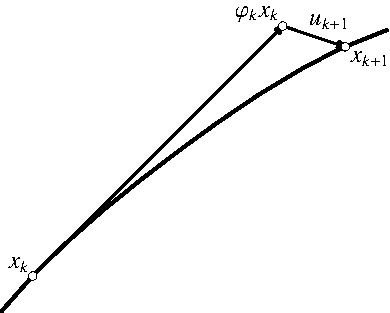
\includegraphics{images/filter-1.pdf}
\caption{Systementwicklung durch die Abbildung $\varphi_k$, der Vektor $u_k$
gibt die Unzulänglichkeiten des durch $\varphi_k$ beschriebenen Modells
wieder.
\label{filter-systementwicklung}}
\end{figure}
In der Realität bewegt sich das System kaum genau nach diesen Gleichungen.
Vielmehr wird es von äusseren Störungen beeinflusst, die sich einer
exakten Vorhersage entziehen, wir tragen dem Rechnung mit Hilfe eines
zusätzlichen Zufallsvektors $u_k$ in den Bewegungsgleichungen
\[
x_{k+1}=\varphi_kx_k+ u_k.
\]
Wir verlangen, dass die Komponenten des Vektors $u_k$ alle unabhängige
Zufallsvariablen sind Erwartungswert 0.
\index{Systemfehler-Kovarianz-Matrix}
\index{Systemfehler!Kovarianz-Matrix}
Die Kovarianz-Matrix $Q_k=E(u_k\cdot u_k^t)$ ist
ein Mass dafür.
$u_k$ heisst auch Prozessrauschen oder Systemfehler.

Die Messfehler modellieren wir durch einen
Zufallsvektor $w_k$, der bei jeder Messung dazukommt, also
\[
z_k=H_kx_k+w_k.
\]
Die Komponenten von $w_k$ sollen unabhängige Zufallsvariablen mit
Erwartungswert $0$ sein, d.~h.~es liegen keine systematischen Messfehler
vor.
Dies bedeutet, dass die Matrix
\index{Messfehler-Kovarianz-Matrix}
\index{Messfehler!Kovarianz-Matrix}
\[
R_k=E(w_kw_k^t)
\]
Diagonalform hat.
Ausserdem sollen die Messfehler unabhängig vom aktuellen Zustand
sein, in Matrix-Form können wir dies durch $E(x_kw_k^t)=0$ ausdrücken.
Man nennt $w_k$ oft auch das Messrauschen.

Die Messfehler $w_k$ und das Prozessrauschen $u_k$ sollen ebenfalls unabhängig
sein, also $E(w_ku_k^t)=0$.

Das Filterproblem besteht darin, aus den bekannten Messwerten von $z_0,\dots,z_k$
die bestmögliche Schätzung $\hat x_k$ zu ermitteln.
Dabei sollen
natürlich die Bewegungsgleichungen berücksichtigt werden.
Da aber
mit der Matrix $R_k$ auch die Grössenordnung der Messfehler bekannt ist,
sollen ``schlechte'' Messwerte geringeres Gewicht erhalten also gute
Messwerte.
Je mehr Werte $z_k$ bekannt werden, desto besser sollte die
Schätzung werden.

In einer praktischen Realisierung muss aber auch die Berechnung der Schätzung
einfach und mit wenig Speicherplatz möglich sein.
Insbesondere sollte zur
Berechnung der neuen Schätzung $\hat x_{k+1}$ nur der letzte bekannte Schätzwert
$\hat x_k$ und die Messung $z_{k+1}$ notwendig sein.
Ausserdem soll der Schätzer
$\hat x_k$ möglichst gut sein, d.~h.~erwartungstreu, linear, iterativ und
mit minimaler Varianz.

\begin{definition}Gegeben ist ein lineares System mit der Zeitentwicklung
\[
x_{k+1}=\varphi_kx_k+u_k,
\]
wobei $x_k$ und $u_k$ unabhängigen Zufallsvariablen sind,
$u_k$ mit Erwartungswert $0$ und bekannter Kovarianzmatrix $Q_k$, d.~h.
\[
E(u_kx_k^t)=0,\qquad E(u_k)=0,\qquad E(u_ku_k^t)=Q_k.
\]
An diesem System werden Beobachtungen
\[
z_k=H_kx_k+w_k
\]
vorgenommen, $w_k$ sind mit $x_k$ und $u_k$ unabhängige Zufallsvariablen
$w_k$ mit Erwartungswert $0$ und bekannter Kovarianzmatrix $R_k$, also
\[
E(w_kx^t)=0,\qquad E(w_k)=0,\qquad E(w_kw_k^t)=R_k.
\]
Das Filterproblem besteht darin, einen Schätzer $\hat x_k$ zu
finden, welcher sich linear aus $\hat x_{k-1}$ und $z_k$ berechnen lässt.
Die Fehler $\tilde x_k=\hat x_k-x_k$ können mit der Fehlerkovarianzmatrix
\[
P_k=E(\tilde x_k\tilde x_k^t)
\]
gemessen werden.
Der Schätzer soll so gewählt werden, dass die Spur
$\operatorname{tr}P_k$ minimal wird.
\end{definition}

\section{Lösung für das Filterproblem}
Zur Zeit $k$ ist das System im Zustand $x_k$, von dem uns aber nur die
Schätzung $\hat x_k$ bekannt ist.
Anschliessend wird sich
das System entsprechend der Zeitentwicklungsgleichung entwickeln und
so den Zustand $x_{k+1}$ erreichen.
Auch diesen Zustand können wir nicht
kennen, es genügt, eine Schätzung davon zu bestimmen.
Dies kann in zwei
Schritten geschehen:
\begin{enumerate}
\item Man überlässt das System sich selbst, und versucht eine möglichst
gute Schätzung für den Zustand $x_{k+1}$ zu finden, die nur auf dem
Wissen zur Zeit $k$ basiert.
Wir schreiben dafür $\hat x_{k+1|k}$.
\item Mit Hilfe der Messung $z_{k+1}$, die zur Zeit $k+1$ stattfindet, wird
$\hat x_{k+1|k}$ zu einer optimalen Schätzung zur Zeit $k+1$ verfeinert.
\end{enumerate}
Tabellarisch können wir die Schritte wie folgt darstellen:
\[
\xymatrix @-1mm {
k\ar[dd]&x_k\ar[dd]\ar[dd]^{\varphi_k, u_k} &\hat x_k\ar[d]^{\varphi_k}      &P_{k} \ar[d]^{\varphi_k,Q_k}    \\
        &           &\hat x_{k+1|k}\ar[d]^{H_k,K_k}&P_{k+1|k}\ar[d]^{R_k,H_k\Rightarrow K_k} \\
k+1     &x_{k+1}    &\hat x_{k+1}  &P_{k+1}
} \]
Die Pfeile sind mit den Matrizen angeschrieben, die bei den einzelnen Schritten zum
Einsatz kommen werden.

\subsection{Voraussage}
\index{Kalman-Filter!Vorhersage-Schritt}
\begin{figure}
\centering
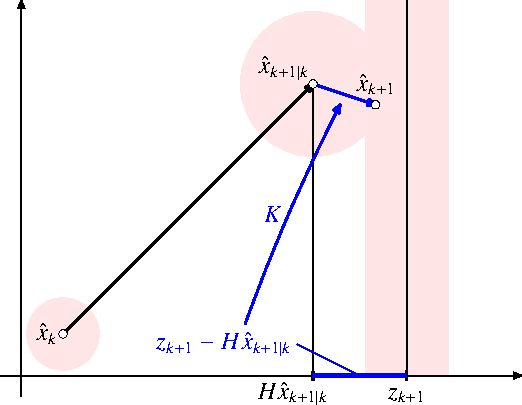
\includegraphics{images/filter-2.pdf}
\caption{Vorhersage und Messung mit ihren jeweiligen Fehlern geben eine
korrigierte Vorhersage höherer Genauigkeit
\label{bild-vorhersage-korrektur}}
\end{figure}
Überlässt man das System sich selbst, wird es sich gemäss der
Entwicklungsgleichung entwickeln.
Allerdings ist uns der Systemfehler
$u_k$ nicht bekannt, die einzige Schätzung, die uns auf der Basis dieser
Informationen möglich ist, ist also
\[
\hat x_{k+1|k}=\varphi_k\hat x_k
\]
In Abbildung~\ref{bild-vorhersage-korrektur} ist die Vorhersage schematisch
dargestellt, zusammen mit ihren Fehlern.

Wir wollen nicht nur $\hat x_k$ zu jeder Zeit bestimmen können, sondern
auch eine Information über die Fehler mitberechnen, also die Fehlerkovarianzmatrix
nachführen.
Wir berechnen daher auch $P_{k+1|k}$
\begin{align*}
P_{k+1|k}&=E(\tilde x_{k+1|k}\tilde x_{k+1|k}^t)\\
&=E( (\hat x_{k+1|k}-x_{k+1} ) (\hat x_{k+1|k}-x_{k+1} )^t)\\
&=E(
(\varphi_k\hat x_k-\varphi_kx_k-u_k)
(\dots)^t
)\\
&=E(
(\varphi_k(\hat x_k-x_k)-u_k)
(\dots)^t
)\\
&=E(
(\varphi_k(\tilde x_k)-u_k)
(\dots)^t
)\\
&=E(
(\varphi_k(\tilde x_k)-u_k)
(\tilde x_k^t\varphi_k^t-u_k^t)
)\\
&=E(\varphi_k\tilde x_k \tilde x_k^t\varphi_k^t)-E(u_k\tilde x_k\varphi_k^t)-E(\varphi_k\tilde x_ku_k)+E(u_ku_k^t)\\
&=\varphi_k E(\tilde x_k \tilde x_k^t)\varphi_k^t-E(u_k\tilde x_k)\varphi_k^t-\varphi_k E(\tilde x_ku_k)+E(u_ku_k^t)\\
&=\varphi_kP_k\varphi_k^t+Q_k
\end{align*}
Damit haben wir einen Formelsatz, mit dem der erste Teilschritt zur Berechnung
der Schätzung zur Zeit $k+1$ möglich ist:
\begin{definition}Der Voraussageschritt für das Filterproblem wird durch
\begin{align}
\hat x_{k+1|k}&=\varphi_k\hat x_k \label{estimate-prediction}\\
P_{k+1|k}&=\varphi_kP_k\varphi_k^t + Q_k \label{covariance-prediction}
\end{align}
berechnet.
\end{definition}

\subsection{Korrektur}
\index{Kalman-Filter!Korrekturschritt}
Im zweiten Schritt wird jetzt aus der provisorischen Schätzung $\hat x_{k+1|k}$
und der Messung $z_{k+1}$ die definitive Schätzung zur Zeit $k+1$ berechnet.
Ebenfalls nachgeführt werden muss die Fehlerkovarianzmatrix $P_{k+1}$.
In Abbildung~\ref{bild-vorhersage-korrektur} ist auch die Korrektur auf der Basis
der Messung $z_{k+1}$ dargestellt, so entsteht eine neue Schätzung
$\hat x_{k+1}$ höherer Präzision.

In den folgenden Herleitungen kommt vor allem der Index $k+1$ vor.
Um die Formeln
etwas zu vereinfachen, erhöhen wir jetzt $k$ um eins, d.~h.~wir können
überall $k+1$ durch $k$ und $k$ durch $k-1$ ersetzen.

Da der Schätzer linear sein soll, und nur von $\hat x_{k|k-1}$ und $z_{k}$
abhängen soll, setzen wir ihn mit Hilfe der zwei Matrizen $K_k'$ und $K_k$
wie folgt an:
\[
\hat x_{k}=K_{k}' \hat x_{k|k-1}+K_{k} z_{k}.
\]
Die Matrizen $K_{k}'$ und $K_{k}$ sollen jetzt so bestimmt werden, dass der Schätzer
$\hat x_{k}$ gute Eigenschaften hat.

Zunächst möchten wir sicherstellen, dass der Schätzer erwartungstreu ist,
oder, was auf das gleiche hinausläuft, dass der Erwartungswert des Fehlers
$\tilde x_{k}=\hat x_{k}-x_{k}$ verschwindet.
Wir berechnen den Fehler
mit Hilfe der Formel für $\hat x_{k}$
\begin{align*}
\tilde x_{k}&=\hat x_{k}-x_{k}\\
&=K_{k}'\hat x_{k|k-1}+K_{k}z_{k}-x_{k}\\
&=K_{k}'\hat x_{k|k-1}+K_{k}H_{k}x_{k} + K_{k}w_{k}-x_{k}\\
&=K_{k}'\hat x_{k|k-1}+K_{k}H_{k}x_{k} -x_{k} + K_{k}w_{k}\\
&=K_{k}'(\tilde x_{k|k-1}+x_{k})+K_{k}H_{k}x_{k}-x_{k}+K_{k}w_{k}\\
&=(K_{k}'+K_{k}H_{k}-I)x_{k}+K_{k}'\tilde x_{k|k-1}+K_kw_k
\end{align*}
Daraus berechnet man den Erwartungswert des Fehlers
\begin{align*}
E(\tilde x_{k})&=(K_{k}'+K_{k}H_{k}-I)E(x_{k})+K_{k}'E(\tilde x_{k|k-1})+K_{k}E(w_{k})\\
&=(K_{k}'+K_{k}H_{k}-I)E(x_{k})
\end{align*}
weil $\tilde x_{k|k-1}$ bereits erwartungstreu ist und $E(w_{k})=0$ nach Voraussetzung.
Dies verschwindet nur dann immer, wenn die Matrix in Klammern $0$ ist,
also
\[
K_{k}'+K_{k}H_{k}-I=0\qquad\Rightarrow\qquad K_{k}'=I-K_{k}H_{k}.
\]
Somit ist $K_{k}'$ durch die Bedingung der Erwartungstreue eindeutig bestimmt.
Mit dieser Wahl von $K_{k}'$ wird der Schätzer jetzt
\[
\hat x_{k}=(I-K_{k}H_{k})x_{k|k-1}+K_{k}z_{k}.
\]

Die zweite Bedingung ist, dass die Fehlerkovarianzmatrix möglichst klein wird,
daher berechnen wir zunächst $\tilde x_{k}$:
\begin{align*}
\tilde x_{k}&=\hat x_{k}-x_{k}\\
&=(I-K_{k}H_{k})\hat x_{k|k-1}+K_{k}z_{k}-x_{k}\\
&=(I-K_{k}H_{k})\hat x_{k|k-1}+K_{k}H_{k}x_{k}+K_{k}w_k-x_{k}\\
&=(I-K_{k}H_{k})\tilde x_{k|k-1}+K_{k}w_k
\end{align*}
Somit ist $\tilde x_{k}$ durch $\tilde x_{k|k-1}$ ausgedrückt, damit sollten
wir $P_{k}$ aus $P_{k|k-1}$ berechnen können:
\begin{align*}
P_{k}&=E(\tilde x_{k}\tilde x_{k}^t)\\
&=E(
((I-K_{k}H_{k})\tilde x_{k|k-1}+K_{k}w_k)
(\dots)^t
)\\
&=(I-K_{k}H_{k})P_{k|k-1}(I-K_{k}H_{k})^t\\
&\quad +(I-K_{k}H_{k})E(\tilde x_{k|k-1}w_k^t)K_{k}^t\\
&\quad+K_{k}E(w_k\tilde x_{k|k-1}^t)(I-K_{k}H_{k})\\
&\quad+K_{k}E(w_kw_k^t)K_{k}^t\\
&=(I-K_{k}H_{k})P_{k|k-1}(I-K_{k}H_{k})^t +K_{k}R_kK_{k}^t
\end{align*}
Diese Formeln bilden nun auch den zweiten Schritt, offen ist nur noch die
geeignete Wahl der Matrix $K_{k}$.
\begin{definition}
Der Korrekturschritt im Filterproblem ist gegeben durch
\begin{align}
\hat x_{k}&=(I-K_{k}H_{k})x_{k|k-1}+K_{k}z_{k} \label{estimate-correction}\\
P_{k} &=(I-K_{k}H_{k})P_{k|k-1}(I-K_{k}H_{k})^t +K_{k}R_kK_{k}^t \label{covariance-correction}
\end{align}
\end{definition}

\subsection{Der optimale Filter}
\index{Kalman-Filter!optimaler Filter}
Die Zeitentwicklung des Schätzers kann nun bis auf die unbekannte Matrix $K_k$
berechnet werden.
Es bleibt, $K_k$ zu bestimmen.
$K_k$ soll so gewählt werden,
dass die Spur von $P_{k}$ minimal wird.
Dabei können wir verwenden,
dass $P_{k}$ von der Form $ABA^t$ ist, wobei $B$ eine symmetrische
Matrix ist.
Für solche Matrizen ist die Ableitung nach den Komponenten
$A$ leicht zu berechnen, das Minimum von $\operatorname{tr}(ABA^t)$
kann daher durch Nullsetzen der Ableitung gefunden werden.

\begin{hilfssatz}Ist $B$ eine symmetrische Matrix und $A$ eine beliebige
Matrix, dann ist die Matrix der Ableitungen von $\operatorname{tr}(ABA^t)$
nach den Komponenten von $A$  ist $2AB$.
\end{hilfssatz}

\begin{proof}[Beweis]
Es ist
\[
\operatorname{tr}(ABA^t)=\sum_{i,j,k}a_{ij}b_{jk}a_{lk}.
\]
Ableiten nach $a_{uv}$ ergibt:
\[
\frac{\partial}{\partial a_{uv}}\operatorname{tr}(ABA^t)
=\sum_{k}b_{vk}a_{uk}+\sum_{j}a_{uj}b_{jv}
\]
Die zwei Terme auf der rechten Seite unterscheiden sich nur durch
die Bezeichnung für die Laufvariable, also
\[
\frac{\partial}{\partial a_{uv}}\operatorname{tr}(ABA^t)
=(2AB)_{uv}.
\]
\end{proof}

Angewendet auf $P_{k}$ bedeutet dies, dass für das optimale $K_k$
\[
-(I-K_kH_{k})P_{k|k-1}H_{k}^t +K_kR_k=0
\]
verlangt werden muss.
Dies kann man nach $K_k$ auflösen und findet
\begin{align*}
0&=-P_{k|k-1}H_{k}^t +K_k[H_{k}P_{k|k-1}H_{k}^t +R_{k}]\\
P_{k|k-1}H_{k}^t&=K_k[H_{k}P_{k|k-1}H_{k}^t +R_{k}]\\
K_k&= P_{k|k-1}H_{k}^t [H_{k}P_{k|k-1}H_{k}^t +R_{k}]^{-1}
\end{align*}
Damit ist das Filterproblem eigentlich vollständig gelöst.
Wir bemühen uns
aber noch, mit der Lösung für $K_k$ die Berechnung der Fehlerkovarianz etwas zu
vereinfachen.
Es gilt
\begin{align*}
P_{k}&=(I-K_{k}H_{k})P_{k|k-1}(I-K_{k}H_{k})^t+K_{k}R_kK_{k}^t\\
&=P_{k|k-1} + K_{k}(H_{k}P(-)H_{k}^t+R_k)K_{k}^t -K_{k}H_{k}P_{k|k-1}-P_{k|k-1}H_{k}^tK_{k}^t\\
&=P_{k|k-1} - P_{k|k-1}H_{k}^t(H_{k}P_{k|k-1}H_{k}^t+R_k)^{-1}H_{k}P_{k|k-1}\\
&=(I-P_{k|k-1}H_{k}^t(H_{k}P_{k|k-1}H_{k}^t + R)^{-1}H_{k})P_{k|k-1}\\
&=(I-K_{k}H_{k})P_{k|k-1}\\
\end{align*}
Damit können wir das Resultat zusammenstellen:
\begin{satz}
Der beste lineare Schätzer für das Filterproblem wird durch die Kalman-Matrix
$K_k$ gegeben, welche mittels
\begin{equation}
K_k=P_{k|k-1}H_k^t(H_kP_{k|k-1}H_k^t+R_k)^{-1}
\label{kalman-gains}
\end{equation}
berechnet wird.
Das Fehlerkovarianz-Update wird mit der Kalman-Matrix
vereinfacht zu
\[
P_k=(I-K_kH_k)P_{k|k-1}.
\]
\end{satz}

\subsection{Datenfluss}
\begin{figure}
\[
\xymatrix @-1mm {
&u_k\ar[r]& *+[o][F]{+}\ar[ddd]_{x_k}&                               \\
&&                   & *+[F]{\varphi_{k-1}}\ar `u^l[ul] [ul]          \\
*\txt{unbeobachtetes System}&&                   & *+[F]\txt{DELAY} \ar[u]       \\
&& *{\bullet}\ar[dd]\ar `r^u[ru] [ru]         &                        \\
\ar@{.}[rrr]&&&\\
*\txt{Messung}&& *+[F]{H_k}\ar[d] & \\
&w_k\ar[r]& *+[o][F]{+}\ar[dd]_<<<<{z_k} &                      \\
\ar@{.}[rrr]&&&\\
&& *+[o][F]{-}\ar[d]_{z_k-H_k \hat x_{k|k-1}} &                               \\
&& *+[F]{K_k}\ar[d]  & *+[F]{H_k}\ar `u^l[ul] [ul]   \\
*\txt{Kalman-Filter}&& *+[o][F]{+}\ar[ddd]_{\hat x_k}  & *{\bullet}\ar[u]\ar[l]\\
&&                   & *+[F]{\varphi_{k-1}}\ar[u]^{\hat x_{k|k-1}}            \\
&&                   & *+[F]\txt{DELAY} \ar[u]       \\
&& *{\bullet}\ar `r^u[ru] [ru] \ar[d]&                     \\
&& \hat x_k          &                               \\
}\]
\caption{Datenfluss im Kalman-Filter\label{datenfluss}}
\end{figure}
\begin{figure}
\[
\xymatrix @-1mm {
*+[F]{H_{k-1}}\ar [rd] & & \\
&*+[F]\txt{Berechne $P_{k-1}$ nach (\ref{covariance-correction})}\ar[ddd]&\\
*+[F]{R_{k-1}}\ar[ur] & & \\
*+[F]{\varphi_{k-1}}\ar[dr] & & \\
&*+[F]\txt{Berechne $P_{k|k-1}$ nach (\ref{covariance-prediction})} \ar[dd] & &\\
*+[F]{Q_{k-1}} \ar[ur] & & \\
&*[F]\txt{\strut Berechne $K_k$ nach (\ref{kalman-gains})} \ar[d] && \\
&*{\bullet} \ar `r^u[r] `u^l[ruuuuuuu]_{\text{erhöhe }k} `l^d[uuuuuuu] [uuuuuu] \ar[d]&&\\
&&&\\
}\]
\caption{Berechnung der Kalman-Matrix\label{k-berechnung}}
\end{figure}
Abbildung \ref{datenfluss} zeigt den Datenfluss für den Kalman Filter.
Im oberen Teil des Diagramms ist das `unbeobachtete' System mit seiner
Zeitentwicklung und den Systemfehlern $u_k$ dargestellt.
Unterhalb der
punktierten Linie folgt die Messung, die Matrix $H_k$ reduziert den Zustand
auf diejenigen Grössen, die durch die Messung zugänglich werden, und es
werden die Messfehler $w_k$ hinzugefügt.
Beide Teile sind nur für die
mathematische Beschreibung des Kalman-Filters notwendig, sie werden
sozusagen von der Natur und den Sensoren realisiert.

Die untere Hälfte zeigt den eigentlichen Kalman-Filter.
Aus einem frühren Zustand $\hat x_{k-1}$ wird mit Hilfe der Matrix
$\varphi_k$ eine provisorische Schätzung $\hat x_{k|k-1}$ erstellt.
Mit der Matrix $H_k$ wird darauf eine Messung simuliert.
Diese wird
mit der tatsächlichen Messung verglichen und die Differenz, verstärkt durch
die Kalman-Matrix $K_k$ zur provisorischen Schätzung hinzugefügt, was
die definitive neue Schätzung $\hat x_k$ für $x_k$ ergibt.

In Abbildung \ref{k-berechnung} ist der Datenfluss für die Berechnung
der Fehlerkovarianzmatrix und der Kalman-Matrix dargestellt.

\subsection{Spezialfälle}
Sind die Matrizen konstant, die das System und den Messprozess beschreiben, 
dann werden im Prozess nach Abbildung \ref{k-berechnung} sowohl $P_k$ also auch
$K_k$ oft gegen konstante Matrizen konvergieren.
In diesem Fall kann man
die Matrix $K=\lim_{n\to\infty}K_n$ vorgängig berechnen, und braucht
in der Implementation des Filters die Berechnung der Fehlerkovarianzmatrix
gar nicht mehr mitzuberechnen. 

Wir betrachten den Spezialfall eines konstanten System mit genau einer
Zustandsvariable,
die auch gemessen wird.
Man erwartet keine Änderung der Zustandsvariable,
die Matrix $\varphi$ ist also die Einheitsmatrix.
Der Voraussageschritt wird
dann zu 
\begin{align*}
\hat x_{k|k-1}&=\hat x_{k-1}\\
P_{k|k-1}&=P_{k-1}+Q,
\end{align*}
die Kalman-Matrix 
\[
K_{k}=\frac{P_{k|k-1}}{P_{k|k-1}+R}=\frac{P_{k-1}+Q}{P_{k-1}+Q+R},
\]
und das Update der Fehlerkovarianz damit zu
\begin{align*}
P_k&=(1-K_k)P_{k|k-1}\\
&=\frac{R(P_{k-1}+Q)}{P_{k-1}+Q+R}
\end{align*}
Diese Gleichung hat tatsächlich einen Fixpunkt, den man durch
Einsetzen von $P=P_k=P_{k-1}$ findet:
\[
P=\frac{R(P+Q)}{P+Q+R}
\quad\Rightarrow\quad
P^2+QP-QR=0
\quad\Rightarrow\quad
P=\frac{Q}2+\sqrt{\frac{Q^2}4+RQ}
\]
Damit kann man nun auch einen geschlossenen Ausdruck für $K$
finden:
\[
K=\frac{1}{1+R\biggl(\displaystyle\frac{Q}2+\sqrt{\frac{Q^2}4+RQ}\biggr)^{-1}}
=\frac1{1+R/P}
\]
Wir beobachten darin folgende Grenzfälle:
\begin{enumerate}
\item Ist $R=0$, also keine Messfehler, dann ist $K=1$.
Da die Vorhersage
$\hat x_{k|k-1}=\hat x_k$ ist, bedeutet dies, dass Abweichungen des Messwertes
von der Vorhersage vollständig in den neuen Messwert übernommen werden,
der Kalmanfilter reproduziert also die Messwerte exakt.
\item Im Grenzfall $Q=0$ erhalten wir $P=0$ und damit auch $K=0$.
Dies
bedeutet, dass der Filter überhaupt nicht mehr auf die Messungen reagiert,
der einmal ermittelte Schätzwert ist bereits die beste mögliche Schätzung.
\item Für einen Zwischenwert ergibt sich ein Wert von $K$ zwischen $0$ und $1$.
Nehmen wir als Beispiel an, dass die Messwerte bei $k_0$ einen Sprung machen,
danach aber konstant sind, dann wird der Schätzwert gegen den neuen Messwert
konvergieren.
Die Abweichung zwischen Messwert und vorhergesagtem Wert wird
in jeder Iteration mit $K$ multipliziert.
Bei einem kleinen Wert von $K$
kann der Filter einer Änderung rascher folgen, dafür wird auch $P$ entsprechend
gross, die Schätzung ist also nicht besonders zuverlässig.
Umgekehrt wird der Filter mit $K$ nahe bei $1$ träge, dafür kann dann auch
$P$ kleiner sein, die Schätzungen des Filters sind präziser.
\end{enumerate}
Auch im allgemeinen Fall eines konstanten Systems kann man erwarten,
dass bei einem Sprung der Inputdaten der Filter eine Abweichung vom
wahren Wert zeigt, welche exponentiell zerfällt.

\section{Beispiel: Positionsmessung und Geschwindigkeit}
In diesem Abschnitt soll gezeigt werden, wie man mit Hilfe der
eben dargestellten Theorie einen Kalman-Filter entwickeln kann.
Er soll folgende Aufgabe lösen:
\begin{quote}
Von einem System wird zehn mal
pro Sekunde die Position mit einer Genauigkeit von $\sigma_z=0.7\text{m}$
gemessen.
Man ermittle aus diesen Messdaten möglichst genau die aktuelle Position
und Geschwindigkeit.
\end{quote}
\subsection{Systembeschreibung}
Wir modellieren das System unter der Annahme, dass die Geschwindigkeit in
ausreichender Näherung konstant ist.
Dazu brauchen wir zwei Zustandsvariablen, den Ort und die Geschwindigkeit.
Die Zustandsvektoren $x_k$ sind also zweidimensionale Vektoren.

Für die Zeitentwicklung verwenden wir die Annahme: über einen Zeitschritt
der Länge $\Delta t$
ändert sich die Geschwindigkeit nicht, die Position wird jedoch 
um das $\Delta t$-fache der Geschwindigkeit geändert.
Die Entwicklungsmatrix $\varphi$ ist daher
\[
\varphi=\begin{pmatrix}
1&\Delta t\\
0&1
\end{pmatrix}.
\]

Die Systemfehler geben wieder, in welchem Mass das System von den Annahmen
abweicht.
Die zentrale Annahme ist, dass die Geschwindigkeit konstant ist, dass es
also keine Beschleunigung gibt.
Da die meisten Systeme auch irgend wann wieder zur Ruhe kommen werden,
dürfen wir annehmen, dass der Erwartungswert der Beschleunigung $0$ ist.
Die Varianz der Beschleunigung wird aber nicht 0 sein, kann uns aber als
Mass für die Systemfehler dienen.
Ist $\Delta a$ die Standardabweichung der Beschleunigung, dann erzeugt
diese einen Geschwindigkeitsfehler in der Grössenordnung von
$\Delta a\cdot \Delta t$, und einen Positionsfehler von der Grössenordnung
$\frac12\Delta a\cdot\Delta t^2$.
Als Systemfehlermatrix können wir daher 
\[
Q=
\begin{pmatrix}
\sigma_x^2&0\\
0&\sigma_v^2
\end{pmatrix}
=
\begin{pmatrix}
(\frac12\Delta a\cdot\Delta t^2)^2&0\\
0&(\Delta a\cdot\Delta t)^2
\end{pmatrix}
\]
verwenden.

\subsection{Messprozess}
Von den Zustandsvariablen des Systems wird nur die Position gemessen,
die Messmatrix ermittelt also die erste Variable des Zustandsvektors:
\[
H=\begin{pmatrix}1&0\end{pmatrix}.
\]
Der Messfehler der Position ist aus der Aufgabenstellung bekannt, die
Messfehlermatrix ist die $1\times 1$-Matrix
\[
R=\begin{pmatrix}
\sigma_z^2
\end{pmatrix}.
\]
Damit ist das System vollständig beschrieben.

\subsection{Filter}
Die Matrizen der Systembeschreibung sind in diesem Problem unabhängig
von der Zeit, wir können daher in den Formeln die Indizes weglassen.

\subsubsection{Initialisierung}
Wir stellen uns vor, dass das System sich zu Beginn der Messung an
bekannter Position, die wir der Einfachheit halber mit $0$ bezeichnen,
aus der Ruhe losgelassen wird.
Zur Zeit $t=0$ ist also der Zustandsvektor bekannt, es ist 
\[
x_0=\begin{pmatrix}0\\0\end{pmatrix}
\]
der Nullvektor.
Da Position und Geschwindigkeit exakt bekannt sind, ist die initiale
Fehlerkovarianzmatrix
\[
P_0=\begin{pmatrix}0&0\\0&0\end{pmatrix}.
\]
Man nennt diese Art der Initialisierung des Filters auch
Fisher-Initialisierung, sie ist in diesem Fall angmessen.

\subsubsection{Vorhersage}
Der Kalmanfilter ermittelt die geschätzte Position und Geschwindigkeit aus
einer Abfolge von Vorhersage- und Korrektur-Schritten.
Für die Vorhersage gelten die Gleichungen
\begin{align*}
\hat x_{k+1|k}&=\varphi \hat x_k\\
P_{k+1|k}&=\varphi P_k\varphi^t + Q.
\end{align*}

\subsubsection{Korrektur}
Der Korrekturschritt bestimmt zuerst die Kalman-Matrix $K_{k+1}$ und
dann daraus die endgültigen Schätzungen für den Zustand
$\hat x_{k+1}$ und die Fehlerkovarianz $P_{k+1}$:
\begin{align*}
K_{k+1}&=P_{k+1|k}H^t(HP_{k+1|k}H^t+R)^{-1}
\\
\hat x_{k+1}&= (I-K_{k+1}H)\hat x_{k+1|k} + K_{k+1}z_{k+1}
\\
P_{k+1}&=(I-K_{k+1}H)P_{k+1|k}
\end{align*}

\subsection{Matlab/Octave Code}
Der Kalman-Filter kann mit wenigen Zeilen Matlab/Octave-Code implementiert
werden.
Die Parameter des Systems sind
\begin{verbatim}
deltat = 0.1;
a = 0.4;
sigmav = a * deltat;
sigmax = 0.5 * sigmav * deltat;
\end{verbatim}
Die Systemmatrizen sind
\begin{verbatim}
phi = [ 1, deltat; 0, 1 ];
Q = [ sigmax^2, 0; 0, sigmav^2 ];
\end{verbatim}
Der Messprozess wird beschrieben durch die Matrizen
\begin{verbatim}
H = [ 1, 0 ];
global sigmaz = 0.7;
R = [ sigmaz^2 ];
\end{verbatim}
Die Konstante \verb+sigmaz+ ist global definiert, weil sie in der
Funktion \verb+messung+ benutzt wird, um Messwerte mit normalverteilten
Messfehlern zu simulieren.

Der Filter wird initialisiert mit
\begin{verbatim}
x = [ 0; 0 ];
P = zeros(2, 2);
t = 0;
tlimit = 30;
\end{verbatim}
Und der eigentliche Filtercode ist
\begin{verbatim}
I = eye(2);
t = 0;
while (t < tlimit)
        # Vorhersage
        xpred = phi * x;
        Ppred = phi * P * phi' + Q;

        # Korrektur
        K = Ppred * H' * pinv(H * Ppred * H' + R);
        z = messung(t);
        x = (I - K * H) * xpred + K * z;
        P = (I - K * H) * Ppred;

        # Zeit
        t = t + deltat;
endwhile
\end{verbatim}
Die Funktion \verb+messung+ muss einen für die Zeit $t$ angemessenen
Messwert liefern.
Die Objekte mit dem Suffix \verb+pred+ bezeichnen Resultate des
Vorhersageschrittes.
Die Funktion \verb+pinv+ berechnet die Pseudoinverse.
Da im vorliegenden Fall das Argument nur eine $1\times 1$-Matrix ist,
könnte man auch die gewöhnliche inverse Matrix nehmen oder direkt
durch das einzige Matrixelement dividieren.

\subsection{Simulationsresultate}
\begin{figure}
\centering
\includegraphics{tacho/graph-1.pdf}
\caption{Kalman-Filter zur Ortsmessung (oben) und Geschwindigkeitsbestimmung
(unten).
Die reale Position ({\color{blue}blau}) wird mit relativ grossem
Fehler gemessen ({\color{green}grün}), doch der Filter ({\color{red}rot})
kann die Position rekonstruieren, und sogar einigermassen brauchbare
Werte für die Geschwindigkeit ableiten.
Ebenfalls dargestellt sind die Diagonalelemente der Fehlerkovarianz,
der Positionsfehler ist allerdings 3-fach überhöht.
\label{tacho-graph}}
\end{figure}
In Abbildung~\ref{tacho-graph} ist eine Simulation des eben entwickelten
Filters dargestellt.
Das System befindet sich von Zeit $t=0$ bis $t=10$ am Nullpunkt, bewegt
sich dann zwischen $t=10$ und $t=20$ mit Geschwindigkeit $1$ in Richtung
zunehmender Positionskoordinate, danach bleibt es bis $t=30$ an Position $10$.
Ausgehend von dieser Bewegung werden dem Filter als Messungen $z_k$ die
Positionen sowie ein normalverteilter Messfehler mit $\sigma_z=0.7\text{m}$
erzeugt.

Da die Messfehler relativ gross sind, ist der entstehende Kalman-Filter
ziemlich träge, er ``traut'' der Messung nicht, und folgt vor allem der
Systementwicklungsgleichung.
Erst einige Sekunden nach $t=10$ akzeptiert der Filter, dass das System
sich jetzt bewegt, die Geschwindigkeitskoordinate des Zustandsvektors beginnt
zuzunehmen.
Auch dauert es nach $t=20$ wieder ein paar Sekunden, bis der Filter
die Geschwindigkeitskoordinate nach $0$ zurückkehren lässt.

Der Filter ermittelt auch die zu erwartende Fehlerkovarianz, sie ist
in Abbildung~\ref{tacho-graph} als hellrote Fläche hinter der
Kurve der gefilterten Daten dargestellt.
Da die angenommenen Systemfehler der Position sehr klein sind, ist auch die
Fehlerkovarianz in dieser Koordinate sehr gering, in der Darstellung
ist der Fehler daher dreifach überhöht dargestellt.
Beim deutlich grösseren Fehler der Geschwindigkeit war dies nicht
nötig.

Man beachte, wie der Fehler zur Zeit $0$ zunächst verschwindet, und
sich dann innerhalb der ersten paar Sekunden auf einen konstanten
Wert einstellt.

\subsection{Tuning}
Dieser erste Versuch eines Kalman-Filters ist möglicherweise für
die vorgesehene Anwendung ungeeignet.
Es stellt sich daher die Frage, wie die einstellbaren Parameter
$\sigma_x$ und $\sigma_v$ verändert werden können,
um ein beabsichtigtes Filterverhalten zu erreichen.

Man beachte, dass $\sigma_z$ kein Tuning-Parameter ist, da $\sigma_z$
den bekannten Messfehler der Positionsbestimmung beschreibt.
Allerdings wird angenommen, dass der Messfehler normalverteilt ist.
Falls diese Annahme nicht zutrifft, kann man $\sigma_z$ modifizieren,
um möglicherweise von der Normalverteilung abweichendes Verhalten
zu berücksichtigen.

Kleine Werte von $\sigma_x$ und $\sigma_v$ bedeuten, dass der Filter
vor allem den Systemgleichungen folgt, und Änderungen der
Messwerte nur sehr träge folgt.
Grosse Werte von $\sigma_x$ oder $\sigma_v$ lassen den Filter vor allem
den Messwerten folgen. 
Als Nebeneffekt sind auch die Geschwindigkeitswerte sehr viel stärker
verrauscht, und kaum brauchbar.

Wählt man $\sigma_v$ besonders klein, zwingt man den Filter, die
Geschwindigkeit nur sehr langsam zu ändern.
Der Filter ist ja konzipiert worden ausgehend von der Annahme,
dass die Geschwindigkeit konstant bleibt, und $\sigma_v$ drückt
die Abweichung von dieser Annahme aus.
Ein grosser Wert von $\sigma_v$ erlaubt dagegen, dass die Geschwindigkeit
sehr schnell den veränderten Messwerten folgt.

Die Grösse $\sigma_x$ beschreibt die Abweichung der Entwicklung
der Position vom Modell.
Ein grosser Wert bedeutet, dass der Filter einer Positionsänderung
folgen kann, auch wenn es keine dazu passende Geschwindigkeitsänderung
gibt.
Der Filter wird ziemlich gut der Position folgen, aber der
Geschwindigkeitswert wird unbrauchbar träge.

\section{Beispiel: Höhenmesser mit Scheitelpunktermittlung}
Modellraketen verwenden oft einen elektronischen Höhenmesser, der die Höhe
barometrisch mit Hilfe eines Drucksensors bestimmt.
Die fliegende Modellrakete
kann in erster Näherung als Massepunkt behandelt werden, der nur unter dem
Einfluss der konstanten Schwerkraft fliegt.
Der Systemzustand besteht
dann aus Höhe $h$, Vertikalgeschwindigkeit $v$ und Beschleunigung $a$.
Die Kinematik beschreibt die zeitliche Änderung mit Hilfe des
Differentialgleichungssystems
\[
\frac{d}{dt}
\begin{pmatrix}
h\\v\\a
\end{pmatrix}
=
\begin{pmatrix}
0&1&0\\
0&0&1\\
0&0&0
\end{pmatrix}
\begin{pmatrix}
h\\v\\a
\end{pmatrix}
\]
Die Entwicklungsgleichung für einen Zeitschritt der Länge $\Delta t$ ist
\[
\varphi=\begin{pmatrix}
1&\Delta t&\frac{\Delta t^2}2\\
0&1&\Delta t\\
0&0&1\\
\end{pmatrix}
\]
Wir nehmen an, dass die Systemfehler, also die Matrix $Q$ ebenfalls diagonal sind,
und alle Komponenten den gleichen Fehler $\sigma^2$ haben, also
\[
Q=\begin{pmatrix}
\sigma^2&0&0\\
0&\sigma^2&0\\
0&0&\sigma^2\\
\end{pmatrix}
\]

Mit dem Drucksensor kann nur die Höhe bestimmt werden, also
\[
H=\begin{pmatrix}1&0&0\end{pmatrix}
\]
und entsprechend ist die Matrix $R_k$ ebenfalls nur eine Zahl, welche
den Messfehler $\varrho^2$ der Messung wiedergibt.

Zur Berechnung der Kalmanmatrix muss die Matrix $HP_{k+1|k}H^t+R$ invertiert werden.
Aber $HP_{k+1|k}H^t$ ist einfach nur die Zahl in der linken oberen Ecke, also
der mittlere quadratische Schätzfehler der Höhe.
Das Produkt $P_{k+1|k}H^t$
ist die erste Spalte der Kovarianzmatrix.
Die Kalmanmatrix ist also die erste
Spalte der Kovarianzmatrix dividiert durch $(P_{k+1|k})_{11}+\rho^2$.

